\documentclass{article}

\usepackage[margin=1in]{geometry}
\usepackage{amsmath}
\usepackage{float}
\usepackage{wrapfig}
\usepackage{graphicx}
\usepackage[makeroom]{cancel}
\usepackage[usestackEOL]{stackengine}
\usepackage{mathtools}
\usepackage[oldvoltagedirection]{circuitikz}
\usepackage{multicol}

\ctikzset{bipoles/length=1.2cm}

\begin{document}


\section{Semiconduttori}
Per studiare le caratteristiche corrente-tensione dei circuiti basati su strutture a semiconduttore, biogna studiare il flusso di carica degli elettroni che si muovono nei materiali.\\
Gli elettroni fanno parte della struttura di un singolo atomo

\subsection{Struttura dell'atomo}

Il \textbf{nucleo} \'e formato da un coglomerato di neutroni e protoni, con carica complessiva positiva, attorno al quale ruotano gli elettroni con carica negativa.

L'\textbf{elettrone} che orbita attorno al nucleo ha una propria energia cinetica. La sua `posizione' deriva dal bilanciamento di due forze:
\begin{itemize}
    \item L'accelerazione centrifuga, che allontana l'elettrone dal nucleo
    \item La fora Coulombiana generata dalle due cariche di segno opposto che \'e inversamente proporzionale al quadrato della loro distanza.
\end{itemize}

Piu `veloce' l'elettrone gira attorno al nucleo pi\'u larga \'e la sua orbita, quindi minore \'e l'energia di legame con i protoni in quanto \'e inversamente proporzionale al quadrato della distanza.
L'elettrone oltre ad avere propriet\'a di natura corpuscolare (cio\'e ha una massa discreta che risponde alla legge della meccanica classica), ha propriet\'a ondulatorie ed inoltre non tutte le orbite sono possibili, e quindi, siccome ad un orbita l' elettrone ha una particolare energia, l'elettrone pu\'o avere solo alcuni valori di energia.

\textbf{L'energia \'e quantizzata}: i livelli di energia permessi sono
\begin{itemize}
    \item diversi per ogni tipo di atomo
    \item distribuiti non continuamente
    \item occupati al pi\'u da due elettroni (con spin opposto) $\rightarrow$ \underline{il numero di elettroni per ogni livello \'e finito}\\
        \textbf{per semplicit\'a} ogni livello pu\'o avere solo un elettrone
\end{itemize}

In un \textbf{sistema in quiete}, non perturvato, gli elettroni tendono spontaneamente ad assumere la posizione ocn il livello di energia inferiore.

Un materiale \'e un insieme di atomi che interagiscono tra di loro cio\`e gli elettroni di un atomo sentono la presenza degli altri atomi attraverso la repulsione e l'attrazione. Le orbite variano perch\`e il bilancio delle forze \'e diverso (pi\'u cariche positive, nuclei, e pi\'u cariche negative, elettroni) e quindi le energie si modificano.

Il sistema costituito da due atomi, per esempio, ha diversi livelli energetici dei due atomi isolati.


Il numero di livelli di due atomi che interagiscono non pu\'o variare in quanto non varia il numero di elettroni; varia soltanto la struttura.

Tipicamente ad ogni livelo energetico di un singolo atomo ne corrispondono due vicini e distinti.

Le propriet\'a rimangono uguali in particolare l'energia \'e discretizzata in livelli in cui pu\'o stare un solo elettrone (coppia di spin opposti)

\subsection{Modello a bande energetiche}

L'interazione di pi\'u atomi provoca l'avvicinamento di rispettivi livelli $\rightarrow$ si forniscono ``Grappoli'' di livelli nel quale c'\'e sempre un alternanza tra regioni ricche di livelli permessi e regioni proibite

\begin{itemize}
    \item \textbf{Modello a bande}: ci sono intervalli in cui c'\'e un elevato numero di livelli tutti discreti
        \begin{itemize}
            \item la distribuzione \textbf{non \'e continua}
            \item ogni manda ha un numero finito di livelli e quindi (siccome le propriet\'a di un singolo atomo valgono ancora) ha un numero finito di elettroni che riempiono varie bande partendo da quelle con poca energia.
            \item \textbf{livello energetico di Fermi}: livello limite al di sotto del quale, in assenza di perturazione, tutti i livelli energetici sono occupati al di sopra del quale tutti i livelli energetici sono vuoti.
            \item la caratteristica di un materiale dipende dalla posizione del livello energetico di Fermi
        \end{itemize}
\end{itemize}

\subsection{Tipologia di un materiale}
Per indurre corrente in un materiale bisogna perturbarlo per poter accelerare gli elettroni $\rightarrow$ la perturbazione varia la velocit\'a degli elettroni che cambiano energia cinetica $\rightarrow$ varia la posizione dell'elettrone che ``salta'' in un altro livello energetico

Per avere corrente, quindi occorre che:
\begin{enumerate}
    \item ci sia energia prodotta da una sorgente esterna
    \item l'energia sia sufficente a far ``saltare'' l'elettrone da un livello ad un altro
\end{enumerate}

\subsection{Materiali conduttori}
Il livello di Fermi cade in una banda permessa $\rightarrow$ la distanza minima di energia necessaria a modificare lo stato energetico degli elettroni (creazione di corrente) \'e la distanza tra due livelli che stanno nella stessa banda ed essendo la banda densa di livelli d'energia necessaria \'e piccola

\subsection{Materiali isolanti}
Il livello di Fermi cade in una banda proibita $\rightarrow$ la quantit\'a minima necessaria a muovere un elettrone \'e la distanza tra l'ultimo livello occupato e il primo libero cio\'e almeno pari al gap energetico

L'energy gap \'e molto pi\'u grande della distanza minima tra due livelli energetici della stessa banda e per questo i materiale isolanti conducono molto pi\'u difficilmente elettroni rispetto a materiali conduttori

Per\'o un materiale isolante pu\'o sempre condurre elettroni ma, al contrario dei materiali conduttori, ha bisogno di pi\'u energia (pari almento all'energy gap)

Si pu\'o notare che un elettrone per potersi muovere deve essere in una banda con alcuni livelli energetici liveri quindi una banda complentamente vuota o completamente piena non d\`a nessun contributo alla corrente.
\begin{itemize}
    \item le bande completamente piene vengono trascurate dall'analisi della corrente in quanto i loto elettroni hanno una remota possibilit\'a di ``saltare'' in un livello energetico libero
    \item la situazione \'e come quella di una bottiglia: il liquido si pu\'o muovere grazie ad una perturbazione se la bottiglia non \'e completamente vuota o piena (il liquido c'\'e ma non ha spazio per muoversi).
    \item Vengono definite le due bande fondamentalmente (quelle a cavallo del livello energetico di Fermi)
\end{itemize}

\textbf{Banda di conduzione}: sopra il livello di Fermi


\textbf{Banda di valenza}: Sotto il livello di Fermi


\subsection{Semiconduttore}
La differenza tra i semiconduttori e gli altri materiali \'e la diversa interazione con il mondo esterno.

Metodi  di perturbazione
\begin{itemize}
    \item \textbf{termica}: (siccome la termperature \'e diversa dallo 0 assoluto, gli elettroni che compongono le molecole dei vari materiali si muovono in funzione della temperatura in modo caotico)
    \item \textbf{ottica}: (n fotone porta una cera energia che viene trasformata da una radiazione)
\end{itemize}

Il livello teorico di Fermi \'e in condizinoe della non perturbazione cio\'e allo 0 assoluto.\\
Nella realt\'a ci sono continui scambi di energia

\begin{itemize}
    \item in un \textbf{isolante} l'energia media scambiata non \'e sufficiente a foar ``saltare'' un elettrone dalla banda di valenza a quella di conduzione
    \item in un \textbf{semiconduttore} il gas energetico \'e paragonabile all'energia scambiata con l'ambiente per un semplice effetto termico
\end{itemize}

\subsection{Caratteristiche del semiconduttore}
\begin{enumerate}
    \item il livello energetico di Fermi cade nella banda proibita
    \item l'energy gap \'e paragonabile all'energia media scambiata con l'ambiente esterno
\end{enumerate}

La probabilit\'a dell'elettrone che riceva un energia pari ad 1 gap \'e elevata in un semiconduttore a temperatura ambiente.

$\rightarrow$ si pu\'o generare corrente in quanto
\begin{enumerate}
    \item l'elettrone (che si troa in un livello energetico pi\'u alto e ha quindi una maggiore energia cinetica $\rightarrow$ maggiore velocit\'a) si trova in una banda con molti livelli energetici vuoti, serve poca energia per farlo saltare in un altro livello energetico (per questo la \textbf{banda} si chiama \textbf{di conduzione} $\rightarrow$ si comporta come un conduttore)
    \item \textbf{la banda di valenza} diventa parzialmente occupata in cui si pu\'o verificare un moto di elettroni con piccola energia
\end{enumerate}

\subsection{Differenza tra un conduttore ed un semiconduttore}
\begin{itemize}
    \item In un conduttore esiste solo una banda parzialmente occupata che costituisce il trasporto di corrente
    \item In un semiconduttore necessariamente esistono due bande entrambe parzialmente occupate $\rightarrow$ questo provoca la caratteristica non lineare
\end{itemize}

\subsubsection{Osservazione}
La quantit\'a di elettroni presenti nella banda di conduzione dipende dalla temperature $\rightarrow$ la conducibilit\'a elettrica consumata all'aumentare della temperatura (in quanto aumenta il n\textsuperscript{o} di elettroni che possono ``saltare'' nella banda di conduzione)
\begin{itemize}
    \item questo effetto \'e utilizzato per i sensori di temperature in quanto $\theta$ \'e funzione della temperature.
    \item questo effetto pu\'o essere pericoloso perch\'e la corrente provoca calore per effetto Joule $\rightarrow$ il componente si autoriscalda
    \item \'e un meccanismo instabile che pu\'o provocare la rottura di un dispositivo (problema dell'elettronica di potenza)
\end{itemize}

\section{Meccanismo di conduzione nei Semiconduttori}
I materiali semiconduttori sono prevalentemente della quarta colonna, della tabola periodica degli elementi.

\begin{itemize}
    \item \underline{Silicio}, Germanio o anche di leghe di materiali della 3\textsuperscript{a} e 5\textsuperscript{a} colonna p
    \item GaAs, Arsenuro di gallio

        InP solfuro di indio
\end{itemize}

Il \underline{silicio} \'e il materiale pi\'u diffuso in natura. Per poterlo utilizzare bisogna lavorarlo in maniera complessa
\begin{itemize}

    \item Gli atomi di silicio si legano tra di loro formando un reticolo regolare. Gli elettroni di valenza (quelli esterni) formano un legame covalente cio\'e gli atomi condividono una coppia di elettroni costituendo un legame forte.
    \item Il silicio ha 4 elettroni di valenza disponibili a stabilire un legame formando una struttura cristallina (reticolo cubico).

        Ogni nucleo ha 4 legami covalenti. Gli elettroni di legame sono quelli pi\'u lontani dal nucleo e quindi con una maggiore energia cinetica ed una minore energia di legame $\rightarrow$ sono nella banda di valenza (occupata dagli elettroni di valenza che fromano i legami con gli altri atomi)
\end{itemize}

In condizione di perturbazione (termica o ohmica) un elettrone pu\'o ricevere energia saltando nella banda di conduzione $\rightarrow$ entra in un livello energetico superiore e quindi ha un orbita pi\'u grande e un minor legame con il nucleo $\rightarrow$ ha bisogno di un ulteriore piccola energia per cambiare il suo nuovo stato orbitale.

In presenza di un campo elettrico esterno ($\overrightarrow{F}=q\overrightarrow{E}$) l' elettrone riesce ad allontanarsi dall'atomo

Il moto dell'elettrone \'e ostacolato dal reticolo cristallino

L'elettrone che dalla banda di valenza entra nella banda di conduzione \'e debolmente legato al suo nucleo e sottto ad una forza esterna (campo elettrico) pu\' facilmente cambiare il suo stato di moto $\rightarrow$ \textbf{elettrone libero} $\rightarrow$ pu\' contribuire alla corrente.

Per il principio di conservazione dalla carica, quando l'elettrone si allontana globalmente la carica totale \'e equilibrata ma localmente no $\rightarrow$ l'assenza di un elettrone comporta uno sbilanciamento di carica positiva $\rightarrow$ il legame vagante \'e il livello lasciato lbero dall'elettrone che \'e andato nella banda di conduzione.

Questo livello livero pu\'o essere facilmente riempito a spese di un picco di energia


\subsubsection{Microscopicamente accade che}
\begin{enumerate}
    \item un elettrone si mjuove in banda di conduzione
    \item tanti elettroni si muovono in piccoli scostamenti (nella banda di valenza) provocando un apparente spostamenteo di una carica positiva nella direzione opposta della carica negativa in banda di conduzione
\end{enumerate}

i meccanismi di conduzione nei semiconduttori sono diverse dal meccanismo di conduzione nei conduttori

\begin{itemize}
    \item \textbf{Nella banda di conduzione}: il \underline{moto} \'e dovuto dallo svincolamento di una \underline{carica negativa} dal nucleo. (livera di muoversi sotto l'effetto di un campo elettrico)

    \item \textbf{Nella banda di valenza}: il \underline{moto} \'e dovuto ad una successione dei piccoli movimenti di elettroni quali corrisponde microscopicamente un moto in direzione contraria di una \underline{carica positiva}


    \item \textbf{Lacuna} (= assenza di carica negativa) corrisponde ad un moto in cascata di diversi elettroni che rappresenta macroscopicamente un moto di un unica particella fittizia dotata di carica positiva

    \item \textbf{Elettrone} viene considerato soltanto l'elettrone livero di muoversi nella banda di conduzioneo
\end{itemize}

In un \textbf{conduttore} esiste un'unica specie di portatori (trasferimento di elettroni)

In un \textbf{semiconduttore} esistono due meccanismi di conduzione $\rightarrow$ carica negativa (elettrone) e carica positiva (lacuna) $\rightarrow$ esistono due specie di portatori di carica

La generazione di un elettrone provoca la nascita di una lacuna

$n$ = n\textsuperscript{o} elettroni per cm\textsuperscript{3}

$p$ = quantit\'a di lacune per cm\textsuperscript{3}

$n=p$ perche il materiale \'e uniforme (Silicio Puro)

\begin{itemize}
    \item L'evento di sumltanea generazione di un elettrone libero o della corrispondente lacuna si chiama \textbf{evento di generazione} di una coppia elettrone-lacuna (coppia $e$-$h$ dove $h$=hole)

        Pu\'o essere provocato sia in maniera elettrica (campo elettrico) che per via ottica (grazie a due fotoni come nelle macchine fotografiche digitali) che per via acustica/meccanica
    \item ci deve essere il fenomeno opposto alla generazione in quanto il sistema \'e costante nel tempo cio\'e l'alterazione pu\'o cedere l'energia in eccesso che aveva liberato e ritornare nella banda di valenza. L'elettrone occupa una lacuna. $\rightarrow$ effetto di ricombinazione

        L'energia viene ceduta sottoforma di di calore o radiazione luminosa (LED)
\end{itemize}

Sapendo che $q=1.602\times10^-14 C$ per conoscere la densit\'a di carica
\begin{itemize}
    \item degli elettroni liberi $\rightarrow$ $-q\times n$
    \item delle lacune $\rightarrow$ $+q \times n$
\end{itemize}

\begin{multicols}{2}
    \textbf{Evento di generazione di una coppia elettrone-lacuna}

    \textbf{$G$ = tasso di generazione}

    \begin{itemize}
        \item \'e il numero di coppie elettrone-lacuna che vengono generati nell'unit\'a di volume e nell'unit\'a di tempo (velocit\'a di generazione)
        \item dipende dalla temperatura

        \item l'elettrone, ricevendo energia si alloontana dal legame covalente creando una lacuna interpretata come una carica positiva in eccesso
    \end{itemize}


    \columnbreak{}
    \textbf{Evento di ricombinazione}

    \textbf{$R$ = tasso di ricombinazione}
    \begin{itemize}
        \item \'e il numero di coppie elettrone-lacuna che si ricombinano nell'unit\'a di volume e nell'unit\'a di tempo
        \item dipende dalla temperatura e dai meccanismi di ricominazione.
        \item un elettrone libero incontra una lacuna, cede energia e occupa lo stato libero di legame.
            L'energia pu\'o essere ceduta sottoforma di energia termica o radiazione ottica
    \end{itemize}

\end{multicols}

Siccome il sistema \'e in una condizione stazionaria $G=R$ perch\'e la velocit\'a con cui vengono generate le coppie \'e uguale a quella con cui vengono ricombinate $\rightarrow$ il tempo di ``sopravvivenza'' della coppia si chiama tempo di vita della coppia

Siccome in condizioni stazionarie $p=n$ possono avere lo stesso nome

$n\textsubscript{i}(T)$ = concentrazione intrinseca di portatori (lacune o elettroni); dipenda in prima approssimazione dalla temperatura (in modo esponenziale)

Valore tipico $n\textsubscript{i}=10^{10} [\frac{coppie}{cm^3}]$ a 300$K$, i.e. 27\textsuperscript{o}C

Densit\'a degli atomi del reticolo cristallino di silicio = $10^{23} [\frac{atomi}{cm^3}]$; \'e estremamente pi\'u grande di $n\textsubscript{i}$ che \'e per\'o sufficente a cambiare completamente il comportamento del dispositivo.

Per poter sfruttare la presenza di lacune ed elettroni bisogna sbilanciare l'equazione $p=n$ cio\'e non bisogna utilizzare silicio puro.

\section{Materiali Estrinseci}
\subsubsection{Atomi Donatori (5\textsuperscript{a} colonna)}

Si introduce nel reticolo cristallino di silicio una piccola quantit\'a di atomi della 5\textsuperscript{a} colonna della tavola periodica degli elementi (ex. Fosforo)

\begin{itemize}
    \item Questi atomi hanno 5 elettroni di valenza
    \item La piccola quantit\'a non influenza la struttura del reticolo
\end{itemize}

L'atomo di Fosforo \'e un atomo drogante e non forma una lega col silicio in quanto la proporzione \'e incongrua: il numero di atomi inseriti deve essere talmente piccolo da non portare perturbazione alla struttura reticolare

\textbf{atomo di Fosforo} $\rightarrow$ quattro elettroni di valenza formano un legame covalente col silicio.

Il \textbf{quinto elettrone} non forma legami, \'e debolmente legato al nucleo e si allontana da esso non crea una lacuna (=posto vacante in un legame covalente).
La carica positiva che si forma (che bilancia la carica negativa che si \'e allontanata) \'e un protone del nucleo, \'e una carica fissa $\rightarrow$ \textbf{il fosforo si ionizza positivamente}

La carica positiva non pu\'o spostarsi, come faceva la lacuna, in quanto nessun legame vacante ha un ``buco'' $\rightarrow$ \textbf{si genera un elettrone ma non una lacuna}

Dal punto di vista energetico la struttura a banda cambio:
l'atomo di fosforo introduce dei nuovi livelli caratteristici della sua natura
\begin{itemize}
    \item la banda proibita per il silicio cambia grazie all'introduzione di qualche molecola di fosforo che aggiungono qualche livello energetico in prossimit\'a della banda di conduzione
    \item l'elettrone che occupa il nuovo livello pu\'o facilmente ``saltare'' nella banda di conduzione senza creare una lacuna nella banda di valenza

\end{itemize}

Il Fosforo \'e un atomo donatore perch\'e ``regala'' un elettrone libero senza modificare la struttura.

N\textsubscript{0} = concentrazione di atomi donatori = $\frac{n\textsuperscript{o}\,di\,atomi\, donatori}{cm^3}$

Siccome la struttura del cristallo deve essere quella del silicio N\textsubscript{0} $<$ densit\'a diegli atomi del reticolo cristallino di silicio e siccome il n\textsuperscript{o} di elettroni \'e spontaneamente n\textsubscript{i} allora
\[
    10^{10} < N\textsubscript{0} < 10^{20}
\]

Quando $N\textsubscript{0}=10^{20}$ non riesce a modificare la struttura del silicio

Siccome l'energia utile per far ``saltare'' l'elettrone dal livello donatore alla banda di conduzione \'e molto piccola alla temperatura ambiente, tutti gli elettroni di quel livello sono gi\'a nella banda di conduzione, quindi $N\textsubscript{0} \approx n$  (cio\'e ogni atomo donatore cede un elettrone, approssimazione quasi esatta)
\[
    N\textsubscript{D} \approx n > p
\] con atomi donatori (5\textsuperscript{a} colonna)

\subsection{Atomi accettori (3\textsuperscript{a} colonna)}
Si introduce nel reticolo cristallino di silicio una piccola quantit\'a di atomi della 3\textsuperscript{a} colonna della tavola periodica degli elementi (BORO)
\begin{itemize}
    \item Questi atomi hanno 3 elettroni di valenza
    \item la piccola quantit\'a non influisce la struttura del reticolo
\end{itemize}

Il legame valente comporta lo spostamento di un elettrone al quale \'e associato ad uno spostamento di una carica virtuale positiva

\textbf{Atomo di Boro}
\begin{itemize}
    \item si genera una lacuna ma non un elettrone mobile
    \item si crea una carica fissa negativa (ione di Boro negativo)
\end{itemize}

Dal punto di vista di energetico il Boro introduce un nuovo livello energetico (livello accettore), vicino alla banda di valenza
\begin{itemize}
    \item questo livello \'e uno stato legato ad una positione cio\'e gli elettroni nel nuovo livello non si spostano
    \item questo nuovo livello ``cattura'' facilmente un elettrone a spese di una piccola energia
    \item la popolazione di lacune \'e maggiore
\end{itemize}

$N\textsubscript{A}$ = concentrazione di atomi accettori = $\frac{n\textsuperscript{o}\,atomi\,accettori}{cm^3}$

\[
    10^{10} < N_{A} < 10^{20}
\]
$N\textsubscript{A} \approx p > n$ con atomi accettori (3\textsuperscript{a} colonna)

\begin{itemize}
    \item Per un materiale \textbf{intrinseco} (solo silicio puro)

        ci sono soo le coppie elettrone-lacuna

        $p=n=n\textsubscript{i}\quad$ e $\quad p \times n = n\textsubscript{i}^2$ $\qquad$ $N\textsubscript{D} = N\textsubscript{A} = 0$

    \item Per un materiale \textbf{estrinseco} (drogato con atomi accettori o donatori)

        $p \neq n \neq n\textsubscript{i} \quad$ e $\quad p \times n = n\textsubscript{i}$

        Densit\'a di carica $\Rightarrow$ \'e dovuta da
        \begin{itemize}
            \item un elettrone libero
            \item una lacuna
            \item atomi donatore inoizzati positivamente perch\'e hanno ceduto un elettone
            \item atomi accettore ionizzati completamente a temperatura ambiete negativamente
        \end{itemize}

        Solo la carica mobile pu\'o produrre corrente

        $p = N\textsubscript{D} \times q - N\textsubscript{A} \times q - n \times q + p \times q$

        In condizioni di equilibrio sia per materiale intrinseche che estrinseche

        $p \times n = n\textsubscript{i}^2$

    \item \textbf{Bozza di dimostrazione di} $p\times n = n\textsubscript{i}^2$

        In condizione di equilibrio stazionario $G=R$

        G \'e funzione della temperatura $G = \alpha (T)$

        R \'e funzione dia della temperatura, sia del numero di elettroni e di lacune (pi\'u elettroni liberi sono presenti e pi\'u \'e alta la probabilit\'a che troviamo una lacuna)

        $R = \beta (T) \times n \times p$

        $G = \alpha (T) = \beta (T) \times n \times p = R$ $\leftarrow$ questa equazione \'e indipendente dal drogaggio del materiale

\end{itemize}

\[
    n \cdot p = \frac{\alpha(T)}{\beta(T)} = \gamma(T) = n_i^2
\]

In condizione di equilibrio ed ad una temperatura finita $\gamma(T)$ \'e una costante indipendente da $N_D$ e $N_A$ e, siccome per $N_D = N_A$, $n \cdot p = n_i^2$, allora $\gamma(T)$ \'e uguale a $n_i^2$, in quanto non varia al variare del drogaggio

$\Rightarrow$ Siccome $ n \cdot p = n_i^2 = \text{cost}$ \underline{in condizioni stazionarie}, aumentando la concentrazione di elettroni, la concentrazione di lacune cala, in quanto: $n = \frac{N_i^2}{p}$

\subsection{Calcolo di $n(N_D, N_A)$ all' equilibrio, con $N_D$ ed $N_A$ costanti}
\begin{itemize}
    \item $N_D$ e $N_A$ non sono variabili nello spazio
    \item A livello globale la carica \'e nulla
\end{itemize}

Siccome il materiale \'e uniforme, la carica locale \'e nulla $\Rightarrow \rho = 0$

\[
\begin{cases*}
    \rho = q(N_D - N_A -n + p) = 0\\
    p = \frac{N_i^2}{n} \rightarrow \text{Perch\'e $n$ \'e all'equilibrio}
\end{cases*}
\]

\[
    N_D - N_A + \frac{n_i^2}{n} - n = 0; \qquad n(N_D - N_A) + n_i^2 - n^2 = 0
\]
\[
    n^2 - n(N_D - N_A) - n_i^2 = 0 \qquad n = \frac{N_D - N_A}{2} \pm \sqrt{\frac{(N_D - N_A)^2}{4} + n_i^2}
\]

Siccome $n$ \'e positivo per definizione:

\begin{center}
    \framebox{$n = \frac{N_D - N_A}{2} +\sqrt{\frac{(N_D - N_A)^2}{4} + n_i^2}$}\\
    \vspace{10px}
    \framebox{$p = -\frac{N_D - N_A}{2} +\sqrt{\frac{(N_D - N_A)^2}{4} + n_i^2}$}
\end{center}

\'E importante la differenza tra $N_D$ e $N_A$ e non il loro valore:
\begin{itemize}
    \item Principio di complementazione
    \item Bisogna rimanere entro certi limiti (non bisogna alterare la struttura cristallina del silicio)
\end{itemize}

Dal punto di vista energetico se c'\'e un atomo accettore e uno donatore:
% placeholder

Questo \'e utile per la realizzazione diversamente drogante:
Prima si droga con un tipo di atomo tutto il materiale e, dove serve, si aggiunge l'altro atomo drogante.

\begin{itemize}
    \item con $N_D = N_A$ allora $ n = p = n_i$
    \item con $N_D \gg N_A$ e $N_D \gg n_i  \quad n = \frac{(N_D - \cancel{N_A})}{2} + \sqrt{(\frac{N_D - \cancel{N_A}}{2})^2 + \cancel{n_i^2}} \rightarrow n \approx N_D$
    \item con $N_A \gg N_D$ e $N_A \gg n_i  \quad p = -\frac{(\cancel{N_D} - N_A)}{2} + \sqrt{(\frac{\cancel{N_D} - N_A}{2})^2 + \cancel{n_i^2}} \rightarrow p \approx N_A$
\end{itemize}

Gli atomi donatori incrementano la popolazione di elettroni e decrementano la popolaizone di lacune

\begin{minipage}[t]{0.45\textwidth}
    \textbf{Materiale estrinseco di tipo N}
    \begin{itemize}
        \item Il silicio \'e drogato con atomi donatori con concentrazione superiore a quella degli atomi accettori
        \item predominano gli elettroni rispetto alle lacune
    \end{itemize}
    ($N_D$ da $10^{14}$ a $10^{20} cm^{-3}$)

    \begin{center}
        \framebox{\Longstack[c]{$N_D \gg N_A, ni$ \\ $n \approx N_D \quad\text{e}\quad p = \frac{n^2}{N_D}$}}
    \end{center}
\end{minipage}
\begin{minipage}[t]{0.5\textwidth}
    \textbf{Materiale estrinseco di tipo P}
    \begin{itemize}
        \item Il silicio \'e drogato con atomi accettori con concentrazione superiore a quella degli atomi donatori
        \item Predominano le lacune rispetto agli elettroni
    \end{itemize}
    \begin{center}
        \framebox{\Longstack[c]{$N_A \gg N_D, n_i$ \\ $p \approx N_A \quad \text{e}\quad n = \frac{n_i^2}{N_A}$}}
    \end{center}
\end{minipage}

\subsection{Effetto di un campo elettrico su un semiconduttore}
Il campo elettrico esercita una forza sulla carica elettrica pari a

$\vec{F} = -q\vec{E}$ (Forza Coulombiana)

$\vec{F} = m\vec{a}$ con $m=9.81\cdot 10^{31}Kg$

$-q\vec{E} - m\vec{a} \quad \Rightarrow \quad \vec{a} = -\frac{q}{m}\vec{E}$

se il campo elettrico \'e uniforme, il moto \'e uniformemente accelerato (accade solo nel vuoto)

L'elettrone all'interno di un materiale urta contro gli altri atomi (Forza attrattiva del nucleo e forza repulsiva deglu altri elettroni)

Il moto dell'elettrone all'interno di un materiale sotto l'effetto di un campo elettroco esterno \'e:



% Appunti di Tue 21 May 2019 02:48:28 PM CEST
\subsection{?}

Potenza
\begin{itemize}
    \item Statica = 0
    \item Dinamica

        $\rightarrow$ Cortocircuito

        $\rightarrow$ Carico
\end{itemize}

\begin{figure}[ht]
    \centering
    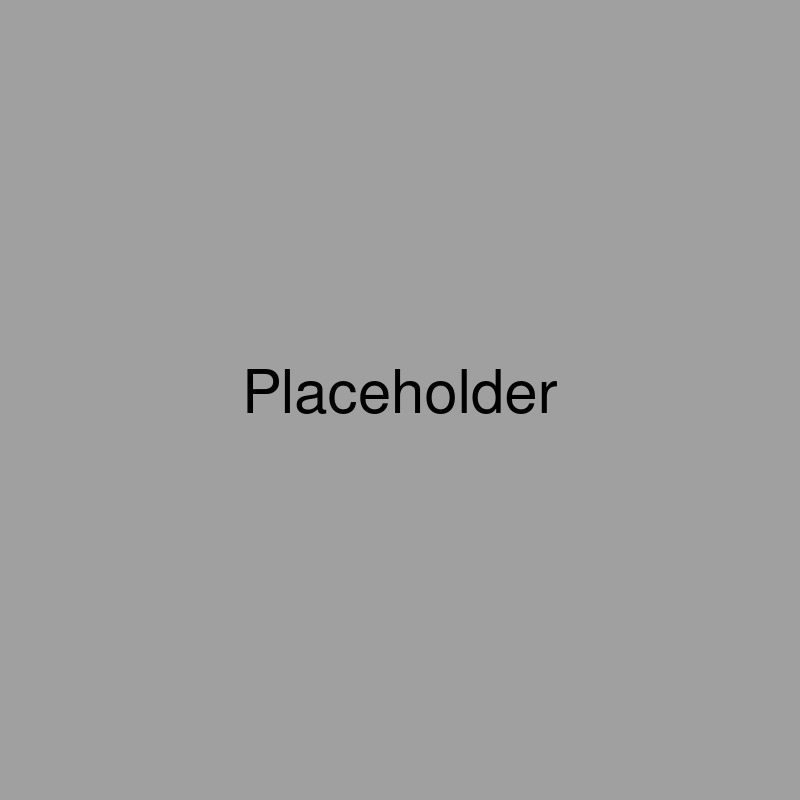
\includegraphics[width=1.8in]{placeholder.jpg}
    \caption{Grafico 1}
\end{figure}

\begin{samepage}
\[
    I_{D} = \frac{\beta}{2}\left\{\frac{t}{t_R} V_{DD} - V_{T} \right\}^2
\]

\[
    V_i(t) = \frac{t_1}{t_r} V_{DD} = V_T \rightarrow t_1 = \frac{V_t}{V_{DD}} t_R
\]

\[
    V_i(t_5) = \frac{t_5}{t_R} V_{DD} = \frac{V_{DD}}{2} \rightarrow t_5 = \frac{t_R}{2}
\]

\[
    \tilde{P} = \frac{1}{T}\int_{0}^{T} V_{DD}I_{D}dt =
    \frac{1}{T} 4 \int_{t_1}^{t_5} V_{DD} \frac{\beta}{2} \left( t \frac{V_{DD}}{t_R} - V_T\right) ^2 dt
\]

\[
    =\frac{4}{T} \frac{\beta V_{DD}}{2} \frac{t_R}{3}
    \left[ \left( t \frac{V_{DD}}{t_R} - V_T\right)^3\right]^{\frac{t_R}{2}}_{\frac{V_T}{V_{DD}} t_R }
\]

\framebox{$\tilde{P_{CC}} = \frac{\beta}{2} \frac{t_R}{T} \left( V_DD - 2 V_T\right)^3$}

% Riprende da ?
\end{samepage}

\begin{figure}[H]
    \centering
    \begin{circuitikz}

        \draw(0, 0) node[eground]{}
        to[Tnmos, n=tnm] ++(0, 1.5)
        to[Tpmos, n=tpm] ++(0, 1.5)
        -- ++(0, 0.2)
        node[vcc]{$V_{CC}$};

        \draw(tnm.G) -- (tpm.G);

        \draw (tnm.D -| tnm.G) to[short, -*] ++(-0.5, 0);
        \draw(tnm.D) -- ++(1, 0)
            to[C] ++(0, -1)
            node[eground]{};

    \end{circuitikz}
    \caption{Circuito 1}
\end{figure}

Applicando Kirkoff: $I_{DP} = I_{Dn} + I_C$

Ricostruita la situazione possiamo analizzare la potenza media associata al carico $\tilde{P_i} = \frac{1}{T}\int_0^T I_{DD} V_{DD} dt $

Sempre dalla relazione di prima, siccome $I_C = 0 \Rightarrow I_{DD} = I_{DP}$


P-mos \'e \textbf{saturo} quando \framebox{$ V_u < V_i + V_t $}

Istantaneamente posso avere un bilancio energetico non nullo, ma in un caso periodico somma dell' energia, per il principio di conservazione deve essere nulla

Sommando le tre potenze devo trovare la potenza complessiva, quindi:
\[
    \tilde{P_L} = \tilde{P_n} + \tilde{P_p} + \tilde{P_C}
\]

\[
    \tilde{P} = \frac{1}{T}\int_0^T  V_U I_C dt = \frac{1}{T} \int_0^T V_U C_L \frac{dV_U}{dt} dt =
    \frac{C_L}{T}\int_{V_U(0)=0}^{V_U(T) = 0} \cdots = 0
\]

Ovvio che \'e nullo perche l'energia di un condensatore \'e legata alla carica

\[
    \tilde{P_P} = \frac{1}{T} \int_0^T V_{BDP} I_{DP} dt = \frac{1}{T}\left[ \int_0^{\frac{T}{2}} V_{BD} I_{DP} dt + \int_{frac{T}{2}}^{2T} V_{SD}I_{DD}dt\right]
\]


\[
    \frac{1}{T} \int_0^{\frac{T}{2}} (V_{DD} - V_U) C_L \frac{dV_U}{dt}dt = -\frac{C_L}{T} \int (V_U - V_{DD}) dV_U = \cdots
\]

\[
    =\frac{C_L}{T} \frac{V_{DD}}{2}^2
\]

Calcolando la potenza consumata dal transitorio di Pull Down (N-mos)
Osservando che nel primo semiperiodo l'n-mos \'e spento, La corrente \'e nulla, quindi ci limitiamo ad integrare nel secondo semiperiodo
\[
    \tilde{P} = \frac{1}{T}\int_0^T  V_U I_C dt = \frac{1}{T} \int_{\frac{T}{2}}^T V_U C_L \frac{dV_U}{dt} dt =
\]

Sapendo che $I_{DD} = -C_L\frac{dV_U}{dt}$ Abbiamo che:

\[
    -\frac{C_L}{T} \int_{V_U(T/2) = V_{DD}} ^ {V_U(T) = 0} V_U \frac{dV_U}{dt} dt = \cdots = \framebox{$\frac{C_L}{T} \frac{V_{DD}^2}{2}$}
\]

Quindi: $\quad \tilde{P_L} = \frac{C_L}{T} {V_{DD}^2} $

Si pu\'o notare che la potenza dissipata non dipende dai parametri dei transitori ($\beta$ non compare nell' espressione)

Siccome quello che mi serve \'e caricare il condendatore, devo spendere un energia doppia rispetto a quella che $\cdots$

Se cambia $\beta$ cambia solo il tempo in cui si carica/scarica il condensatore, $\beta$ non influisce sull'energia

$ \frac{1}{T} = f  \Rightarrow  f C_L {V_{DD}}^2$

Questa che \'e una potenza dinamica, aumenta con la frequenza $\rightarrow$ devo caricare e scaricare il condensatore pi\'u volte

In $P_{CC}$ Compare il rapporto  $\frac{t_R}{T}$, supponendo di essere capaci di far andare pi\'u veloce il circuito, il rapporto tende a rimanere costante $\rightarrow$ Ridurre il periodo aumenta la potenza associata a carica-scarica, ma ha un effetto limitato sulla potenza di cortocircuito

La frequenza sicuramente cresce perche siamo sicuri di riuscire a fare dispositivi pi\'u veloci, ma fare dispositivi piu piccoli, lo scopo della riduzione delle geometrie non \'e fare lo stesso circuito pi\'u piccolo, ma per poter mettere pi\'u ``roba'' all'interno dello stesso chip.

Viene sfruttata la possibilit\'a di mettere pi\'u componenti nello stesso spazio, la frequenza di clock dipende anche dall'architettura e da come \'e fatto il circuito

\begin{figure}[ht]
    \centering
    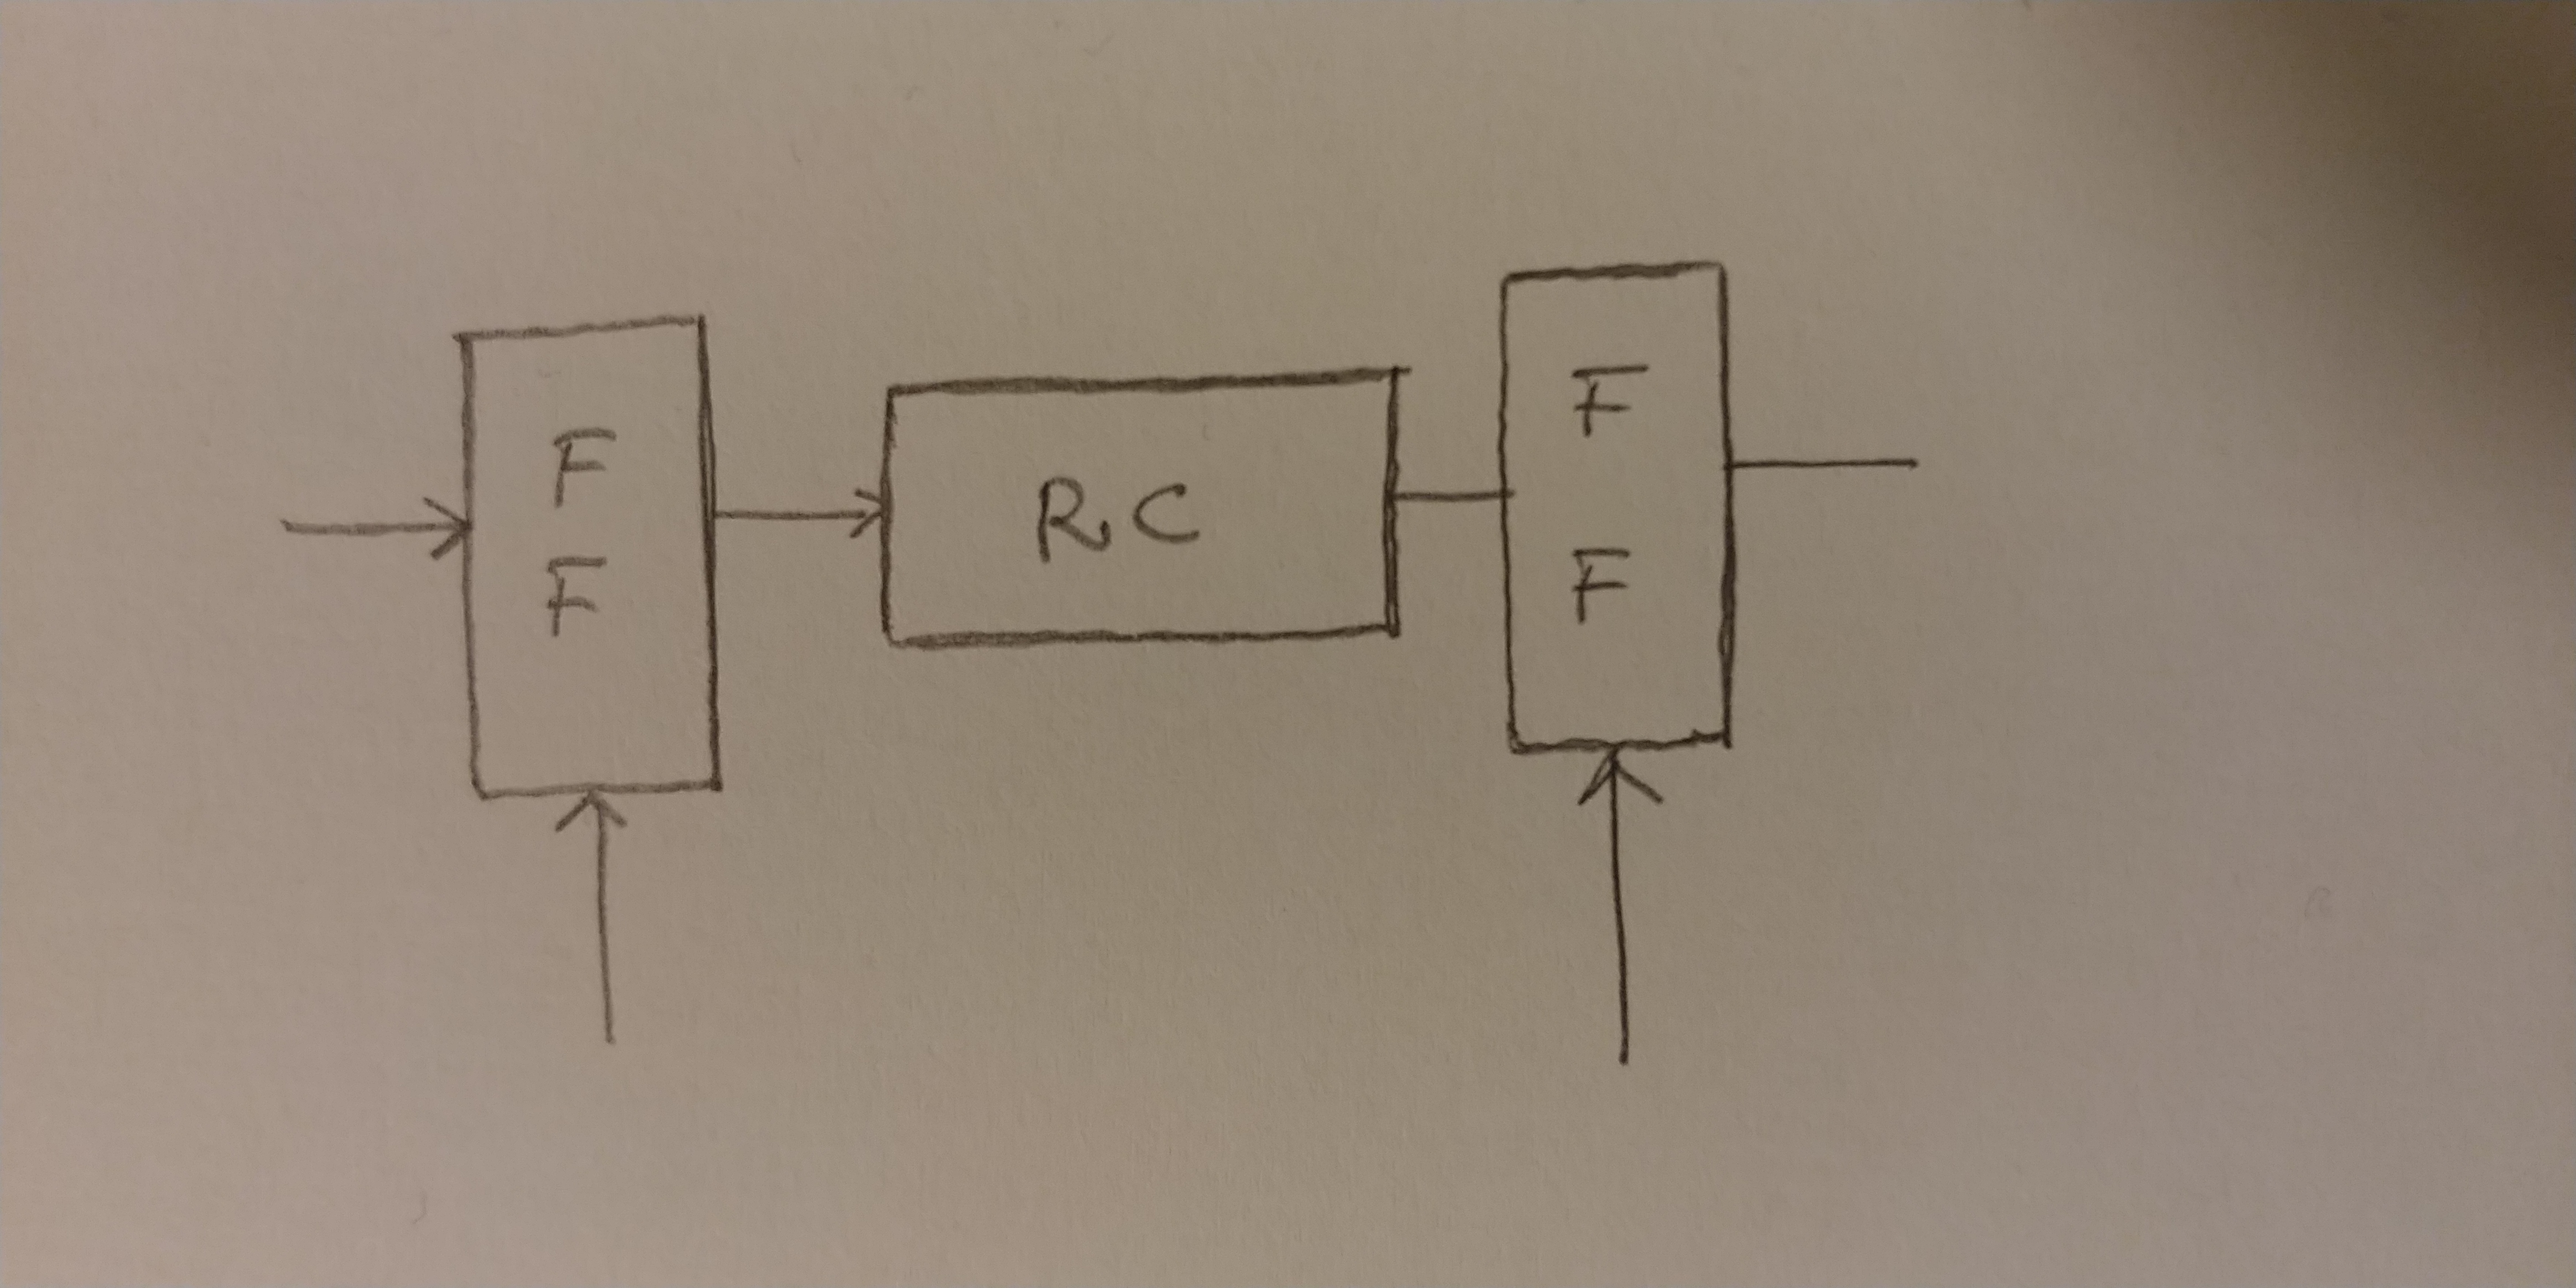
\includegraphics[width=3in]{img/elettronica/esempio_clock.jpg}
    \caption{Esempio di clock}
\end{figure}

Rete sincrona \'e piu robusta e piu sicura al problema delle Alee, il periodo di clock deve garantire che tutta la rete combinatoria, abbia il tempo di completare il suo lavoro.

La possibilit\'a di integrare circuiti pi\'u complessi viene sfruttata per implementare architetture con maggiori prestazioni, es. Circuiti in Parallelo

Siccome abbiamo scoperto che la frequenza di clock impatta direttamente sulla frequenza associata al carico, e tende ad aumentare con la riduzione delle dimensioni, comporta al fatto che, se tutto il resto rimanesse costante, tutto va pi\'u veloce e consuma di pi\'u perche va piu veloce: Utilizzo architetture con maggiore prestazione a cui \'e associato un maggiore consumo

Circuiti c-mos caratterizzato da un basso consumo di potenza statico, ma un alto consumo dinamico

Differenza fondamentale con la logica RTL era che quella consumava sia che lavorasse, sia che non lavorasse

Logica di tipo \textbf{ratioless}: Le dimensioni del transistore non impattano sulla funzionalit\'a

% Lezione del Wed 22 May 2019 03:45:35 PM CEST
\subsection{Immunit\'a ai disturbi in sistemi analogici}
Principale differenza tra elettronica analogica e digitale \'e  che \'e in grado di distinguere il segnale dal rumore.

\begin{figure}[ht]
    \centering
    \begin{circuitikz}
        \draw(-1, 3) node[nmos] (N1){};
        \draw(1, 3) node[nmos, xscale=-1] (N2){};
        \draw(N1.G) to[short, -o] ++ (-0.2, 0) node[above]{$V_1$};

        \draw (0, 0) node[eground] (G){}
            to[isource] ++ (0, 2) node(bisection){} -- ++ (-1, 0) -- (N1.S);
        \draw (N1.D) to[short, -o] ++ (0.5, 0)
            node[above]{$V_U$};

        \draw(1.2, 1) node[anchor=east]{$\big\uparrow I_0$};
        \draw(N1.D) to[R, -o] ++(0, 2)
            -- ++ (0, 1)
            -- ++ (1, 0)
            node(UB){}
            -- ++ (1, 0)
            -- ++ (0, -1)
            to[R, o-] (N2.D);

        \draw(bisection.center) -- ++ (1,0) -- (N2.S);
        \draw(N2.G) to[short, -o] ++ (0.2, 0) node[above]{$V_2$};

        \draw(UB.center) to[short, ->] ++ (0, 1) node[vdd]{$V_{DD}$};
    \end{circuitikz}
    \caption{Amplificatore Differenziale\label{circuito_1}}
\end{figure}


Osservazioni su Figura~\ref{circuito_1}:
\begin{itemize}
    \item Per Kirkoff $ I_1 + I_2 = I_0$

    \item Siccome la somma delle correnti \'e non nulla, i due transistori ($M_1$  e $M_2$), non possono essere spenti allo stesso tempo

        $I_{D\text{sat}} = \frac{\beta}{2}{(V_{GS}-V_T)}^2$

    \item La caratteristica del generatore di corrente sul piano Tensione-Corrente \'e che \'e costante $\Rightarrow$ la tensione $V_X$ \'e incognita

    \item
        Per Kirkoff:
        $V_1 - V_{GS1} + V_{GS2} - V_{2} = 0 \Rightarrow$
        $V_1 - V_2 = V_{GS1} - V_{GS2}$
\end{itemize}

Supponenedo che per ipotesi: $M_1$ se acceso \'e saturo e $M_2$ Se acceso \'e saturo, e, supponendo che $V_1 = V_2$, allora:

$V_1 - V_2 = 0 \Rightarrow V_{GS2} - V_{GS2} = 0 \Rightarrow V_{GS1} = V_{GS2} $

Siccome la corrente dipende solo da $V_{GS}$, se le tensini sono uguali, le correnti sono uguali $\xrightarrow{SAT} I_1 = I_2$

Siccome $I_1 + I_2 = 0 \Rightarrow I_1 = \frac{I_0}{2} , I_2 = \frac{I_0}{2}$

\[
    V_{U1} = V_{DD} - RI_1 = V_{DD} - R\frac{I_0 }{2}
\]

\[
    V_{U2} = V_{DD} - RI_2 = V_{DD} - R\frac{I_0 }{2}
\]
Il valore di uscita non dipende dall'ingresso, se $V_1$ e $V_2$ sono uguali tra di loro, l'uscita non dipende da loro (Se lavoriamo in regione di saturazione)

Questo tipo di circuito non vede il rumore, siccome entra uguale in entrambi gli ingressi

\vspace{20px}
Supponendo ora che $V_1$ e $V_2$ siano \textbf{diversi}, (es $V_1 > V_2$):

\[
    V_1 - V_2 > 0 \Rightarrow V_{GS1} - V_{GS2} > 0 \Rightarrow V_{GS1} > V_{GS2}
\]
\[
    V_{GS1} > V_{GS2} \Rightarrow I_1 > I_2
\]

Dato che la somma delle correnti \'e limitata ($I_1 + I_2 = I_0$), la corrente $I_1$ continua a crescere, mentre $I_2$ diminuisce, Fino a quando la corrente $I_0$ gira unicamente su un ramo. La corrente non pi\'o diventare negativa perch\'e andrebbe contro le condizioni del transistore.

\begin{figure}[ht]
    \centering
    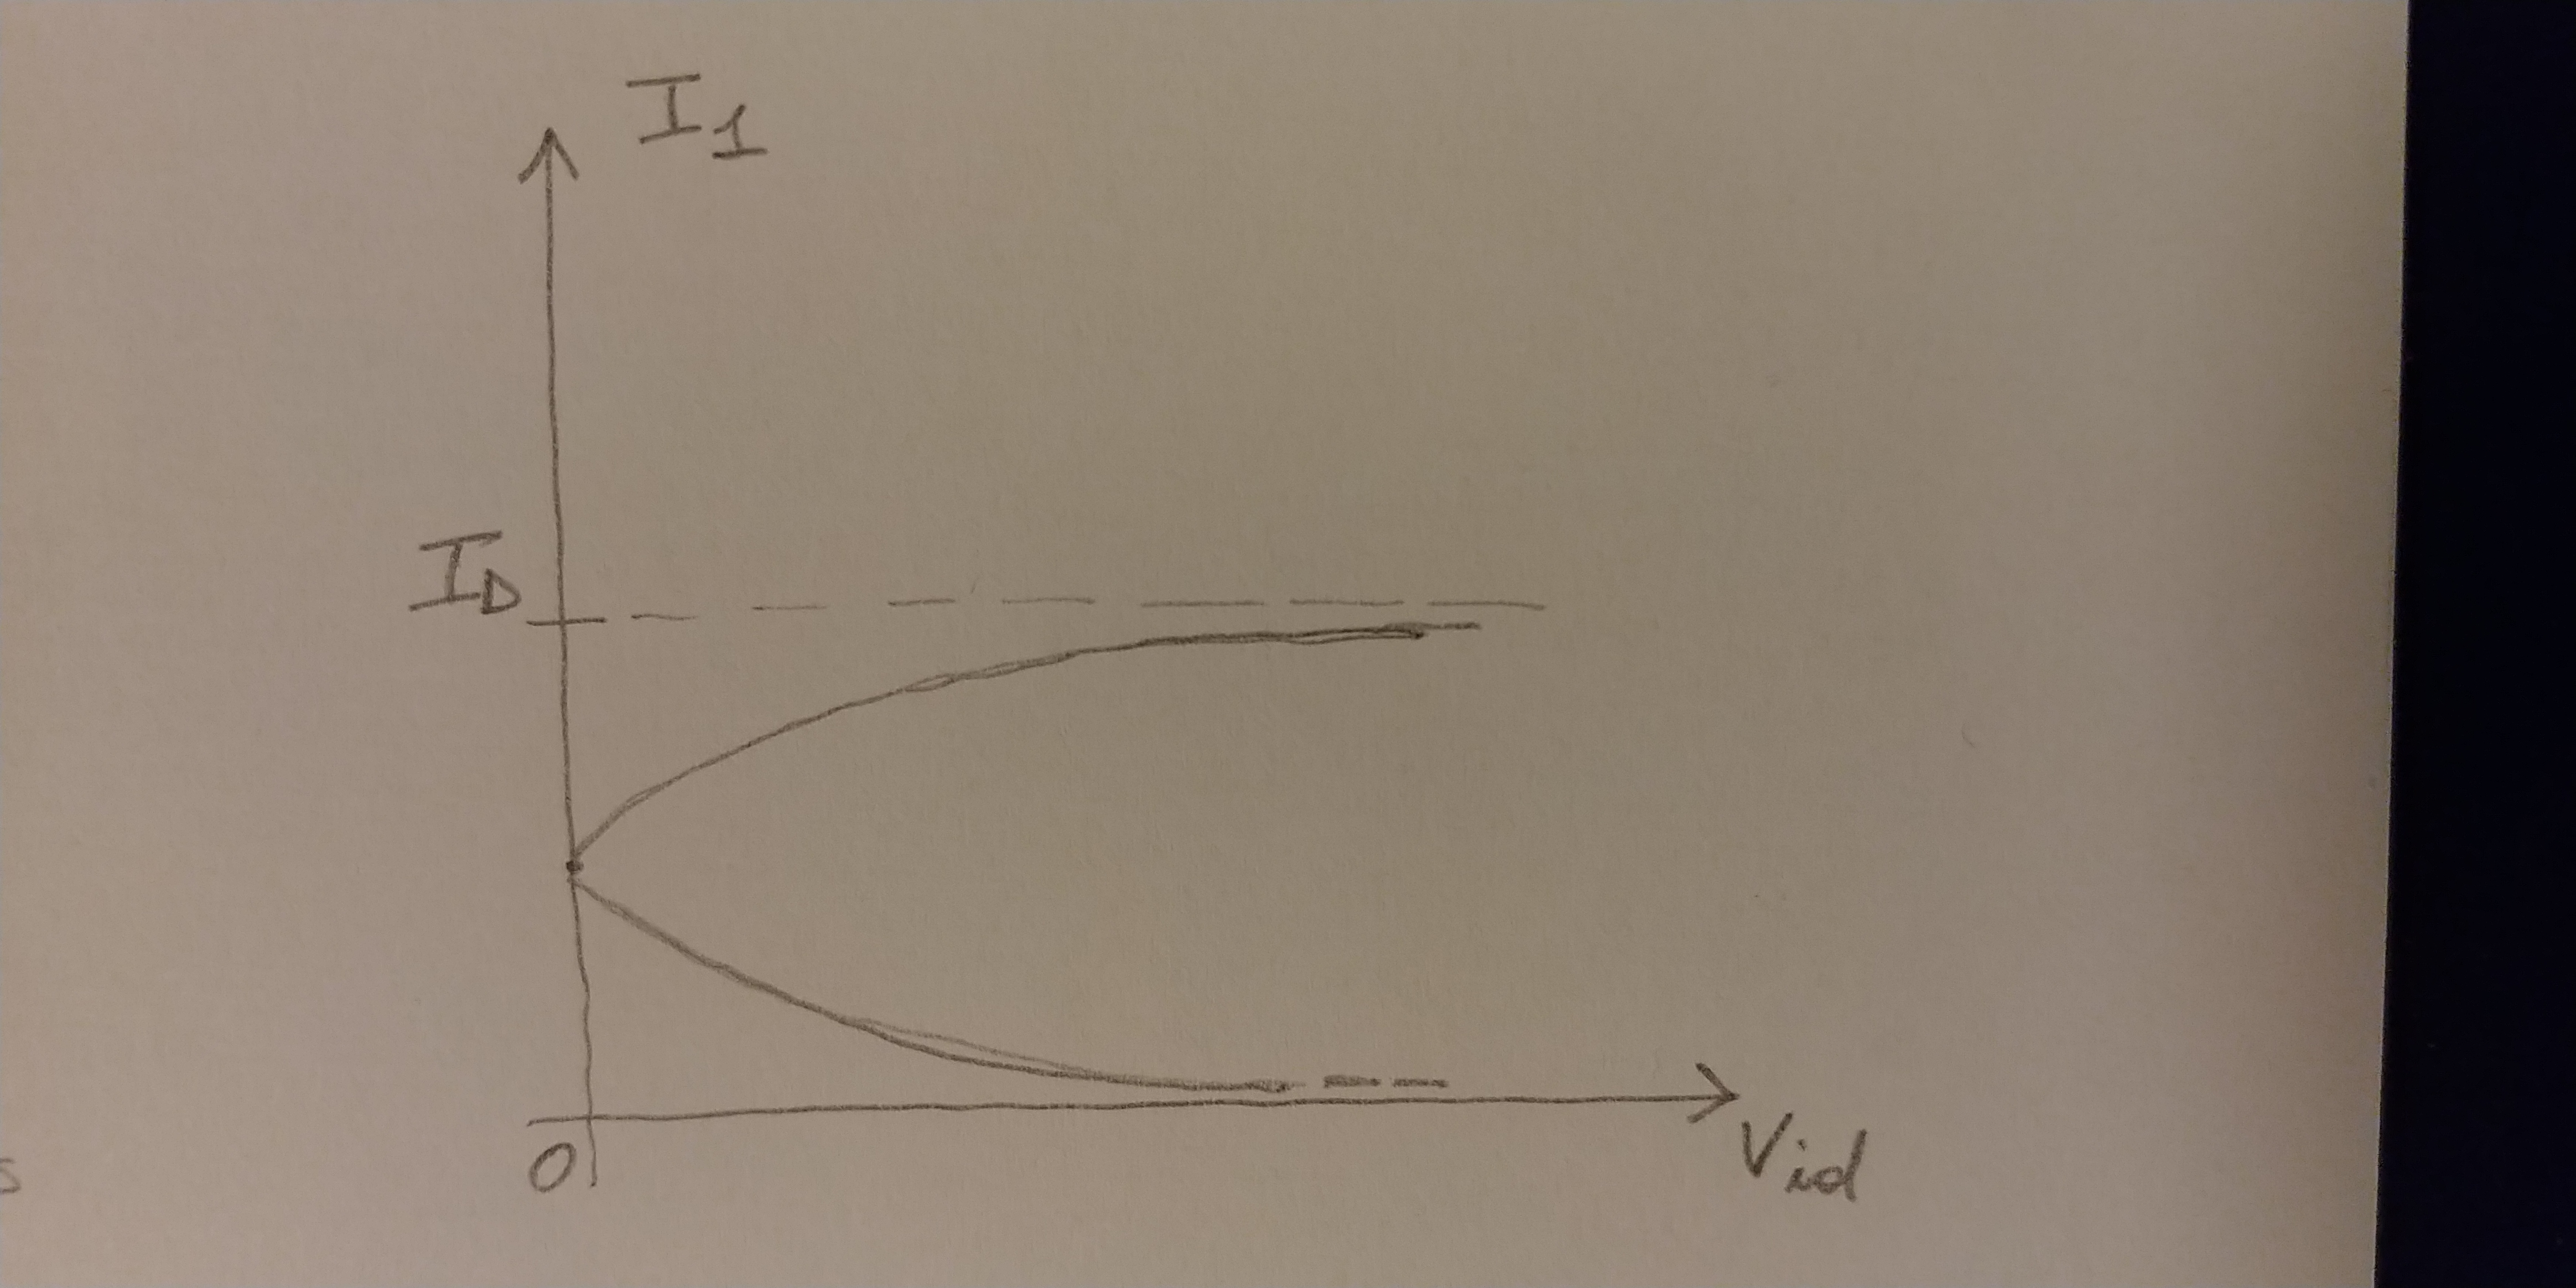
\includegraphics[width=4in]{img/elettronica/grafico2.jpg}
    \caption{Grafico $I_0$, $V_{id}$\label{grafico_analog}}
\end{figure}

Chiamata $V_{iD}$ la tensione differenziale, posso tracciare l'andamento di $I_1$ (Figura~\ref{grafico_analog}), il quale satura al valore $I_0$

\begin{minipage}[t]{0.45\textwidth}
\[
    \begin{cases}
    V_{u1} = V_{DD} - RI_1\\
    V_{u2} = V_{DD} - RI_2
    \end{cases}
\]
\end{minipage}
\begin{minipage}[c]{0.5\textwidth}
    % Grafico
    \begin{center}
        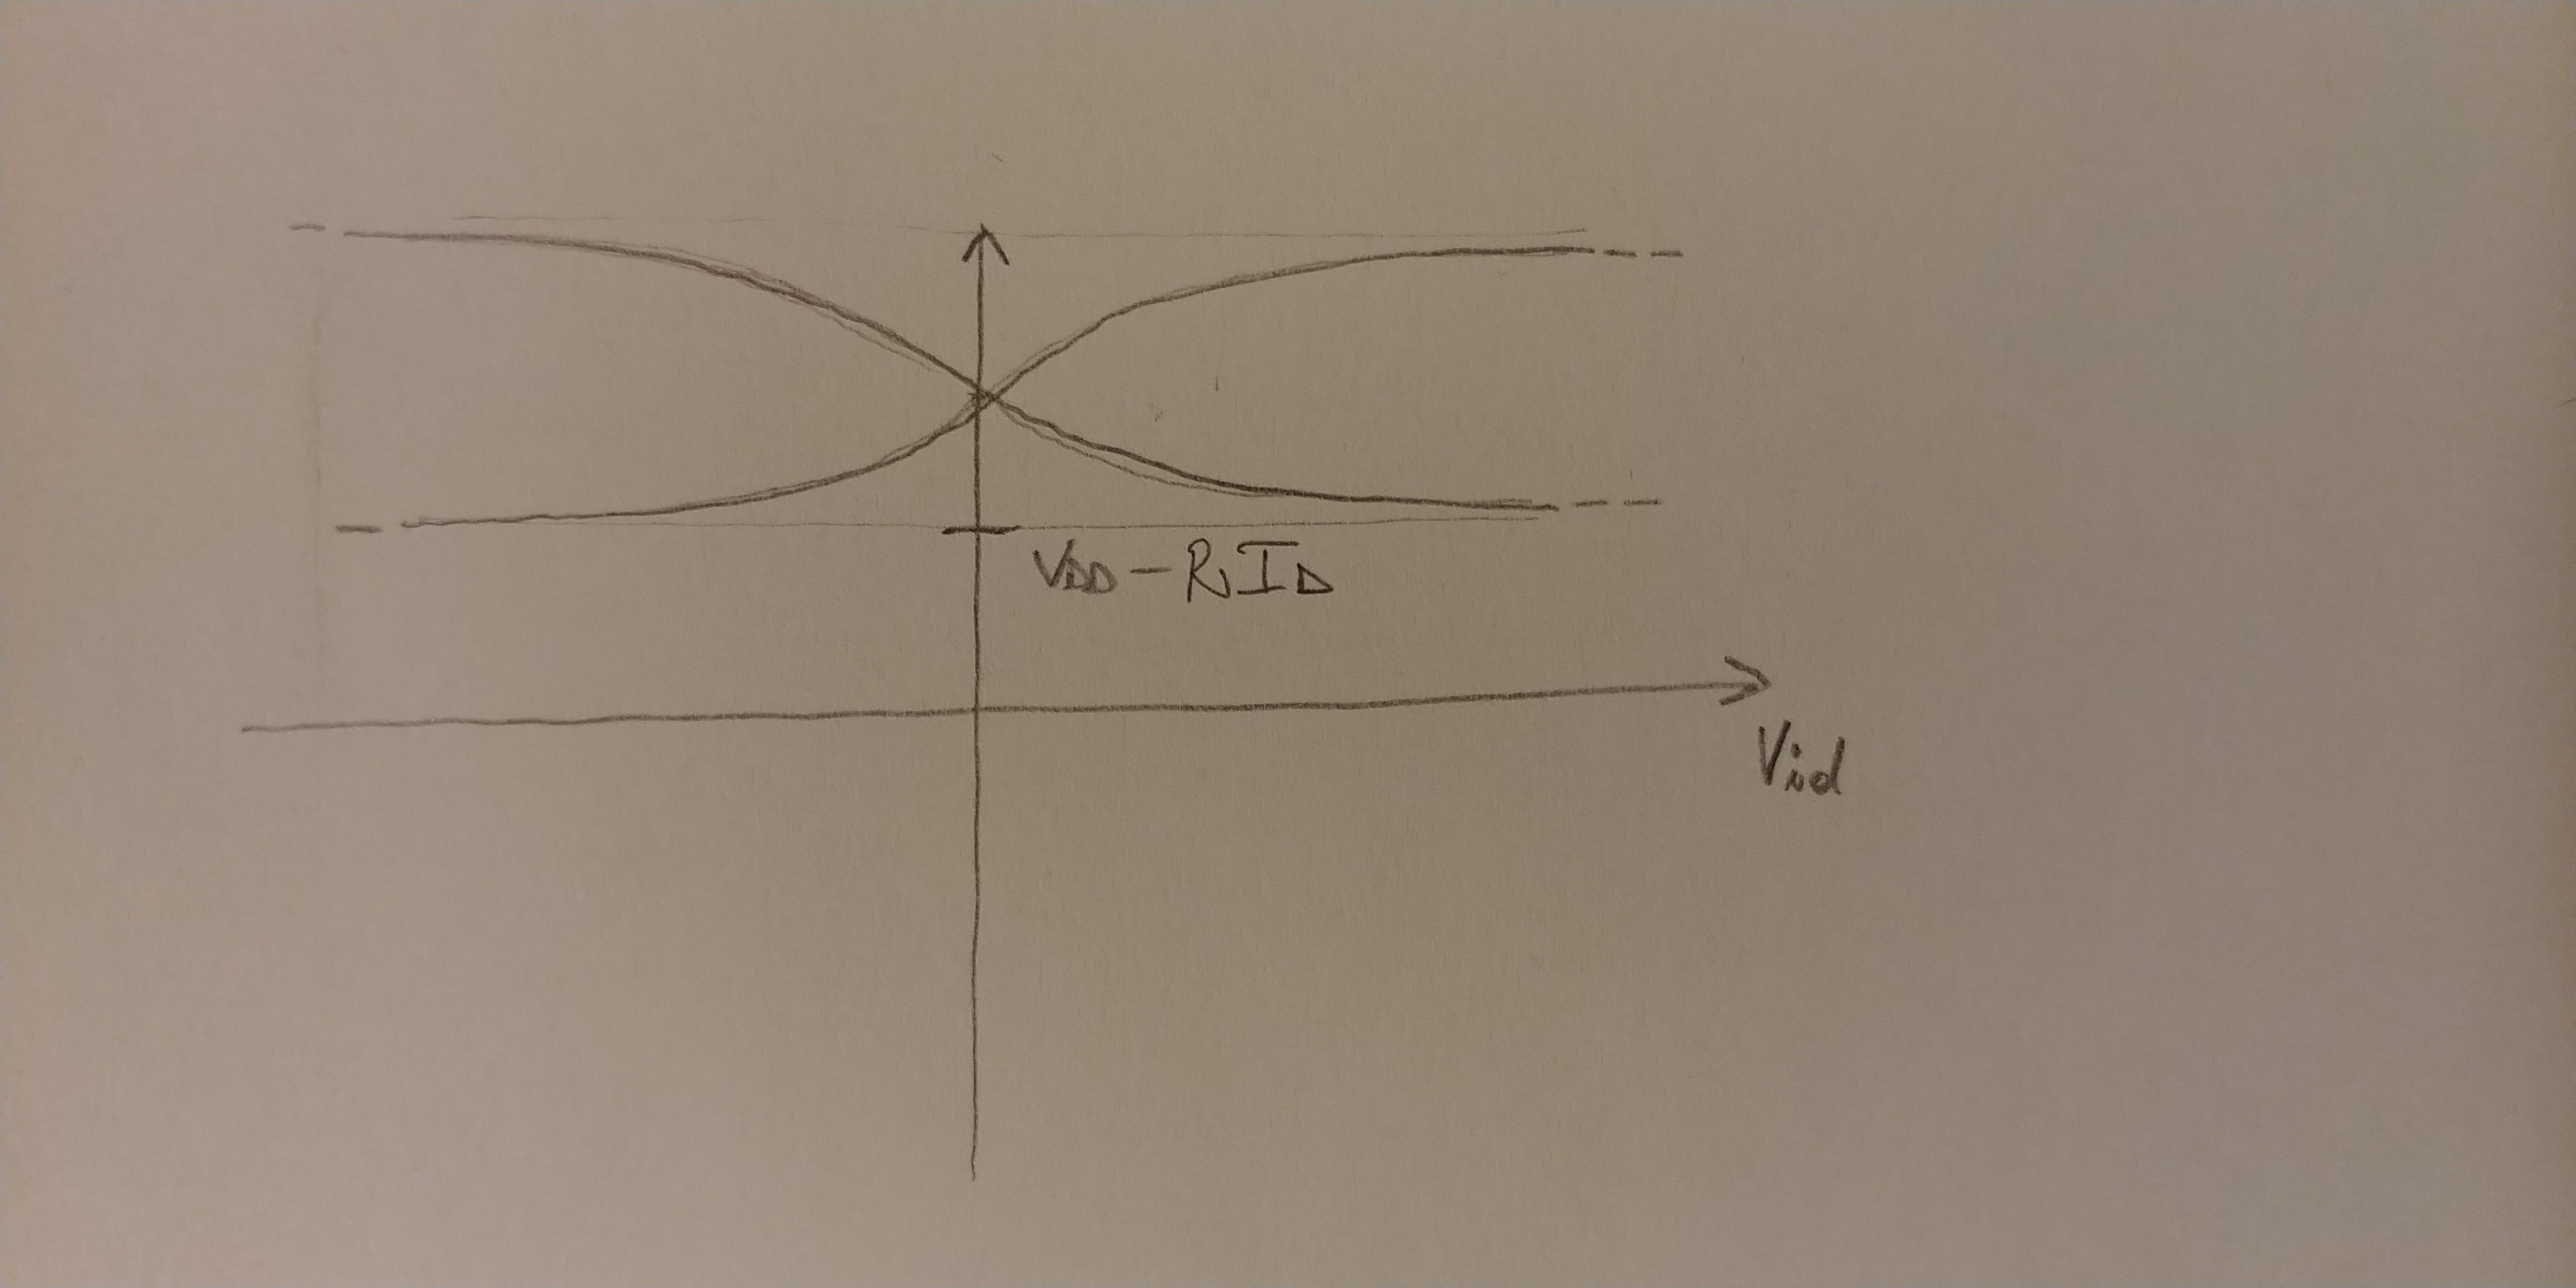
\includegraphics[width=2.8in]{img/elettronica/grafico3.jpg}
    \end{center}
\end{minipage}

Comportamento radicalmente diverso se i segnali variano simultaneamente o non; Quelle non simultanee vengono amplificate

Segnale d'ingresso di modo differenziale
\[
    \begin{cases}
        V_{id} = V_1 - V_2\\
        V_{ic} = \frac{V_1 + V_2}{2}
    \end{cases} \Rightarrow
    \begin{cases}
        V_1 = V_{ic} + \frac{V_{id}}{2} \\
        V_2 = V_{ic} + \frac{V_{id}}{2} - V_{id} = V_{ic} - \frac{V_{id}}{2}
    \end{cases}
\]

Qualunque coppia di segnali \'e suddivisiile in un segnale di modo comune ed un segnale differenziale, questo circuito cancella il segnale di modo comune, mentre il segnale di modo differenziato viene amplificato.

\'E utile per distinguere quale segnale contribuisce all'uscita

\begin{figure}[ht]
\begin{circuitikz}
    \draw(0, 0) node[nmos](Q){};
    \draw(0, -1) node[eground](G){};
    \draw(Q.G) to[short, -o] ++(-0.5, 0) node[above]{$V_i$};

    \draw(Q.D) to[R, -o] ++(0, 2)
        (Q.S) to[-] (G.center);
    \draw(Q.D) to[short, -o] ++(1,0)
        node[above]{$V_u$};
\end{circuitikz}
\end{figure}

Se mettessi in ingresso due volte lo stesso segnale all'amplificatore differenziale (Figura~\ref{circuito_1}):
\[
    V_{ic} = \frac{V_{i0} + \cancel{V_m \sin wt} + V_{i0} - \cancel{V_m \sin wt} - V_{i0}}{2} = V_{i0}
\]

\[
    V_m = \cancel{V_{i0}} + V_m \sin wt - \cancel{V_{i0}} + V_m \sin wt = 2 V_m \sin wt
\]

\subsection{Generatore di corrente}

\begin{figure}[ht]
    \centering
    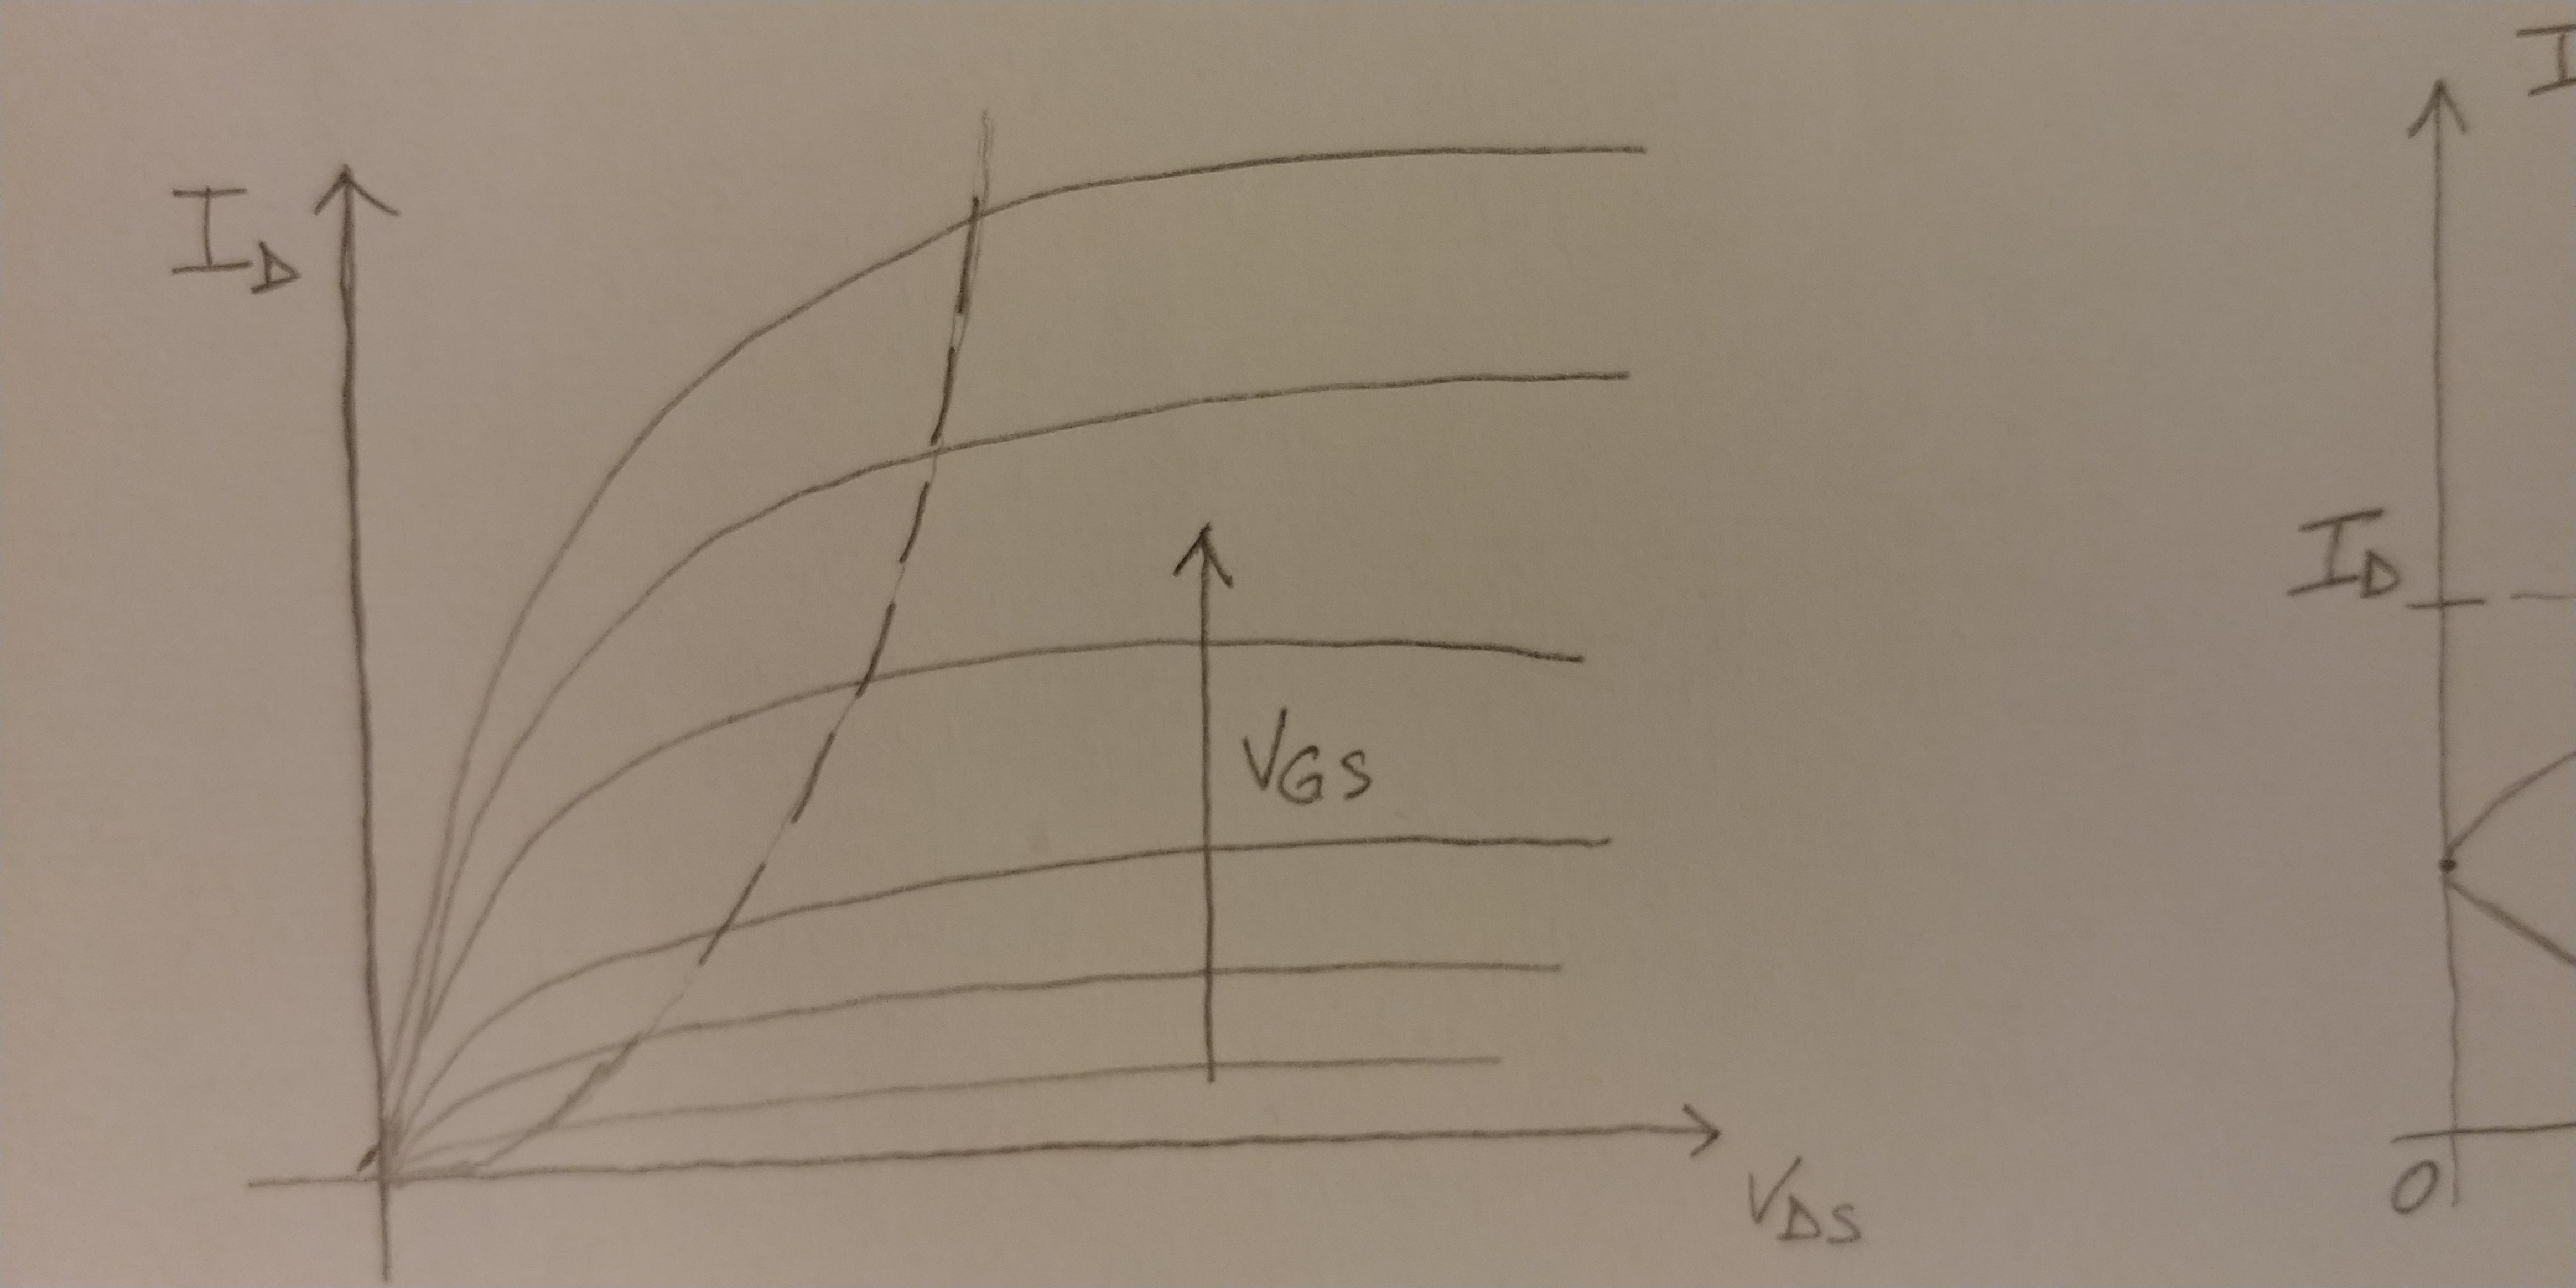
\includegraphics[width=4in]{img/elettronica/grafico1.jpg}
    \caption{Grafico con linee orizzontali}
\end{figure}

Un transistore che lavora in saturazione, genera un uscita costante

Applicando una tensione costante, il transisotre \'e saturo e la corrente vale $I_D = \frac{\beta}{2}(V_{GG} - V_T)^2$

Per tensioni sufficentemente grandi: $V_{GS} < V_{DS} + V_T \Rightarrow V_x > V_{GG} - V_T$ lavora in saturazione




\begin{figure}[H]
    \begin{circuitikz}
        \draw node[ground](G){}
            to[R, -*, l=$R_2$] ++(0, 2) node[anchor=east](VGG){$V_{GG}$}
            to[R, -*, l=$R_1$] ++(0, 3) node[anchor=east]{$V_{DD}$} ;
        \draw (VGG) -- +(1.5, 0) node[nmos, anchor=G](N){};
        \draw(N.center) node[anchor=west]{$\Big\downarrow I_D$};
        \draw (N.D) to[short, -*] ++(0, 0.5) node[anchor=west]{$V_x$};
        \draw (N.S) -- ++(0, -0.2) node[eground]{};

    \end{circuitikz}
    \centering
    %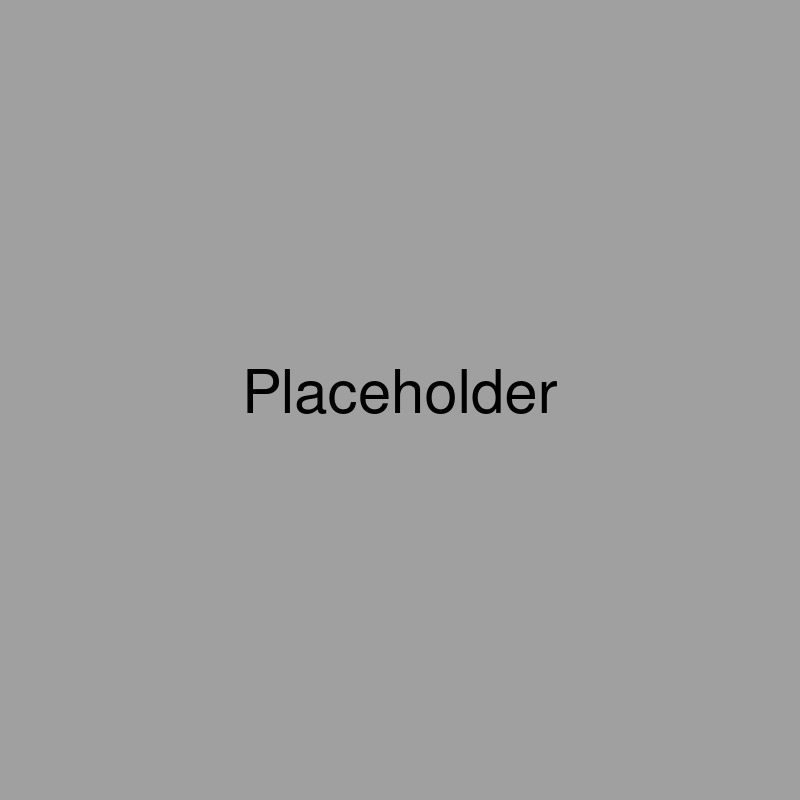
\includegraphics[width=1.8in]{placeholder.jpg}
    \caption{Disegno transitore allungato}
\end{figure}

Per partitore di tensione:
\[
    V_{GG} = V_{DD} \frac{R_1}{R_1+R_2}
    = V_{DD} \frac{1} {1+\frac{R_2}{R_1}} \leftarrow \text{Compare ancora il rapporto tra fattori di forma}
\]

\begin{minipage}{0.45\textwidth}
\begin{figure}[H]
    \centering
    \begin{circuitikz}
        \draw node[ground](G){}
            node[nmos, anchor=D, yscale=-1, xscale=-1](M2){}
            to[] (M2.S) to[R, -*, l=$I_D$] ++(0, 2);


        \draw (M2.G) -- +(1, 0) node[nmos, anchor=G](N){};
        \draw(N.center) node[anchor=west]{$\Big\downarrow I_D$};
        \draw (N.D) to[short, -*] ++(0, 0.5) node[anchor=west]{$V_x$};
        \draw (N.S) -- ++(0, -0.2) node[eground]{};

        \draw (M2.S) to[short, *-] ++(1.5, 0)
            coordinate(angle)
            to[short, -*] (angle |- N);
    \end{circuitikz}
    \centering
    \caption{Disegno transitore allungato 2\label{ta_2}}
\end{figure}
\end{minipage}
\begin{minipage}{0.5\textwidth}
    \begin{figure}[H]
        \begin{circuitikz}
            \draw(0, 0) node[eground](G){}
            node[nmos, anchor=S, xscale=-1](M2){};

            \draw(M2.D) node[nmos, anchor=S, xscale=-1](M3){};
            \draw(M3.D) to[short, -*] ++(0, 1)
            node[right]{$V_{DD}$};

            \draw(M3.D) to[short, *-] ++(1, 0)
            coordinate(angle1) to[short, -*] (angle1 |- M3.G) -- (M3.G);

            \draw(M2.D) to[short, *-] ++(1, 0)
            coordinate(angle2)
            to[short, -*] (angle2 |- M2.G);

            \draw(M2.G) -- ++(0.5, 0)
            node[nmos, anchor=G](M1){};
            \draw(M1.S) node[eground]{};
            \draw(M1.D) to[short, -*] ++(0, 0.5) node[right]{$V_u$};
        \end{circuitikz}
        \centering
        \caption{Figura Dubbia\label{ta_3}}
    \end{figure}
\end{minipage}

Avendo connesso il gate del transistore al Drain
$ \Rightarrow V_{GS2} = V_{DS2} \xrightarrow{V_T > 0} V_{GS2} < V_{DS2} + V_t$

$M_2$ SAT
$M_1$ SAT

\[
    \begin{rcases}
        I_{D2} = \frac{\beta}{2}{(V_{GS2} = V_t)}^ 2\\
        I_{D1} = \frac{\beta}{2}{(V_{GS1} = V_t)}^ 2
    \end{rcases}
    \Rightarrow I_{D1} = I_{D2}
\]


% sep
\[
    \begin{cases*}
        I_D = I_{D2}\\
        I_R = \frac{V_{DD} - V_{GS2}}{R}
    \end{cases*}
    \Rightarrow \frac{V_{DD}  - V_{GS2}}{R} = \frac{\beta}{2} (V_{GS2} - V_T)^2
\]

\[
    I_{D3} = \frac{\beta_3}{2}(v_{GS3} = V_t) ^ 2
\]

Da cui:
\[
    \begin{split}
    \frac{\beta_2}{2}(V_{GS2} - V_T) ^2 = \frac{\beta_3}{2}(V_{GS2} - V_T) ^2\\
    \sqrt{\frac{\beta_2}{\cancel{2}}(V_{GS2} - V_T) ^2}= \sqrt{\frac{\beta_3}{\cancel{2}}(V_{GS2} - V_T) ^2}\\
    \cdots
    \end{split}
\]
\[
    V_{GS2} = \frac{V_{DD} + V_T(\theta - 1)}{\theta + 1}\qquad \left(\theta\coloneqq \sqrt{\frac{\beta_2}{\beta_3}}\right)
\]

Ricordiamo che \'e vero solamente se entrambi i transitori lavorano in \textbf{saturazione}:

\begin{center}
$M_1$ Saturo $\Rightarrow \quad V_{GS1} < V_{DS1} + V_T$

$V_1 - \cancel{V_x} < V_{u1} - \cancel{V_x} + V_T \qquad \rightarrow \framebox{$V_{u1} > V_1-V_T$}$

$M_2$ Saturo $\cdots \quad \Rightarrow \framebox{$V_{U2} > V_2-V_T$}$
\end{center}

Siccome voglio che queste due condizioni siano verificate sempre, il prodotto $RI_0$ \'e costante, Fissato $V_{DD}$, se non devo scendere troppo, vuol dire che impone un vincolo sul valore massimo $RI_0$
\end{document}
